\hypertarget{sec:4}{%
\section{Evaluation Protocol}\label{sec:4}}

\hypertarget{sec:4-1}{%
\subsection{Questions and Materials}\label{sec:4-1}}

We evaluate controlled App detection (RQ1), the contribution of semantic references (RQ2), normal alarms and evidence availability (RQ3), and the increment from a linked Browser (RQ4). Table~\ref{tab:materials} defines each study's denominator and role. Each study's reported rates summarize outcomes across its recorded evaluation positions. Because the studies have different development histories and may overlap in source records or analysis ranges, we report them separately.

% Single-column materials table remains next to Section 4.1 discussion.
% Current manuscript Table 2. Source: input_markdown/sections/04_evaluation_protocol.md.
% Delta/N are count semantics, not accuracy or outcome symbols.
\begin{table*}[t]
  \caption{Evaluation materials and their roles. Counts are record positions, not independent physical devices.}
  \label{tab:materials}
  \centering
  \small
  \setlength{\tabcolsep}{4pt}
  \renewcommand{\arraystretch}{1.12}
  \begin{tabularx}{\textwidth}{@{}>{\raggedright\arraybackslash}p{0.105\textwidth} >{\raggedright\arraybackslash}p{0.195\textwidth} >{\centering\arraybackslash}p{0.055\textwidth} >{\centering\arraybackslash}p{0.055\textwidth} >{\raggedright\arraybackslash}X@{}}
    \toprule
    Material & Subset & $\Delta$ & $N$ & Role and evaluation boundary \\
    \midrule
    \textbf{Controlled} & App & 126 & 252 & Disjoint held-out positions\textsuperscript{a} \\
    \midrule
    \multirow{3}{*}{\textbf{MTC}} & Discovery & --- & 630 & Training-side constraints and tree training \\
      & Historical development & --- & 144 & Historical evaluation with development exposure \\
      & Historically reserved & --- & 117 & Historical evaluation; not a newly blinded cohort \\
    \midrule
    \multirow{3}{*}{\textbf{Specialist}} & Memory & 18 & 48 & Fixed checks; 6 no-effect operations excluded \\
      & Timezone & 6 & 30 & Includes 6 normal system changes \\
      & Geometry & 6 & 66 & Includes 6 normal layout changes; not integrated \\
    \midrule
    \textbf{Paired} & App--Browser & 14 & 46 & 60 development-used positions: pilot 18 + matched 42 \\
    \bottomrule
  \end{tabularx}
  \par\vspace{2pt}
  \parbox{\textwidth}{\footnotesize\raggedright
    $\Delta$ = effective modifications; $N$ = normal records.\enspace
    \textsuperscript{a}\,Controlled App: 14 manipulation recipes $\times$ 3 repetitions $\times$ 3 environments.}
\end{table*}


% Register the wide RQ1 table early so it floats to the following page.
\ifHGMatrix
% Table 3: grayscale detection symbols retain the original grouped outcomes.
% Source: baseline_source/overleaf/tables/01_app_matrix.tex; total-rate-miss rows retained.
\begin{table*}[t]
  \caption{Controlled benchmark positions: detections among nine effective modifications per original recipe; parentheses show nonzero differences from Integrated App. Only identical complete six-method state-count vectors are grouped; recipe counts retain weights. Ablations are separately refitted.}
  \label{tab:app}
  \centering
  \small
  \setlength{\tabcolsep}{4pt}
  \renewcommand{\arraystretch}{1.12}
  \begin{tabularx}{\textwidth}{@{}l c *{6}{>{\centering\arraybackslash}X}@{}}
    \toprule
    Modification group & Recipes & Integrated App & No MTC cap & Web-only & No memory & No timezone & App tree \\
    \midrule
    CPU + memory & 1 & \HGFull\,9 & \HGFull\,9 & \HGNone\,$0\;(-9)$ & \HGNone\,$0\;(-9)$ & \HGFull\,9 & \HGNone\,$0\;(-9)$ \\
    \addlinespace[2pt]
    Screen metrics & 1 & \HGPartial\,6 & \HGFull\,$9\;(+3)$ & \HGPartial\,6 & \HGPartial\,6 & \HGPartial\,6 & \HGNone\,$0\;(-6)$ \\
    \addlinespace[2pt]
    Timezone; plugins/MIME & 2 & \HGFull\,9 & \HGFull\,9 & \HGFull\,9 & \HGFull\,9 & \HGFull\,9 & \HGNone\,$0\;(-9)$ \\
    \addlinespace[2pt]
    Shared detections$^{\dagger}$ & 8 & \HGFull\,9 & \HGFull\,9 & \HGFull\,9 & \HGFull\,9 & \HGFull\,9 & \HGFull\,9 \\
    \addlinespace[2pt]
    Webdriver; WebGL IDs & 2 & \HGNone\,0 & \HGNone\,0 & \HGNone\,0 & \HGNone\,0 & \HGNone\,0 & \HGNone\,0 \\
    \midrule
    \textbf{Total detections} & 14 & \textbf{105/126} & \textbf{108/126} & \textbf{96/126} & \textbf{96/126} & \textbf{105/126} & \textbf{72/126} \\
    Detection (\%) & --- & 83.3 & 85.7 & 76.2 & 76.2 & 83.3 & 57.1 \\
    Missed & --- & 21 & 18 & 30 & 30 & 21 & 54 \\
    \bottomrule
  \end{tabularx}
  \par\smallskip
  \begin{minipage}{\textwidth}\footnotesize
  Tested detections: \HGFull\ all nine; \HGPartial\ $0<d<9$; \HGNone\ none.
  $^{\dagger}$Playwright, Puppeteer, CDP multi-field, and Stealth presets; platform-only, UA-only, UA-plus-platform, and language-list edits.
  All methods: 0/252 controlled-normal alarms and zero U, FAILED, and EMPTY\_MODEL on these held-out positions.
  Saved results: \textsc{retention} for rule models, \textsc{fitted} for the tree. Three extra no-cap screen detections carry a separate normal-record cost (Table~\ref{tab:normals}).
  \end{minipage}
\end{table*}

\fi

% Float registration for the specialist table, placed near RQ2 in the PDF.
% Table 4: grouped fixed checks; symbols encode observed detection counts only.
% Source: input_markdown/sections/05_results.md.
\begin{table}[t]
  \caption{Fixed specialist comparisons. Normal denominators include six system changes (Timezone) and six layout changes (Geometry). U and FAILED are zero. Six no-effect memory operations are excluded from 18 effective modifications and 48 normals.}
  \label{tab:specialists}
  \centering
  \small
  \setlength{\tabcolsep}{3pt}
  \renewcommand{\arraystretch}{1.12}
  \begin{tabularx}{\columnwidth}{@{}>{\raggedright\arraybackslash}X >{\centering\arraybackslash}p{0.21\columnwidth} >{\centering\arraybackslash}p{0.17\columnwidth}@{}}
    \toprule
    Fixed check & \makecell{Detected /\\modified} & \makecell{Normal\\alarms} \\
    \midrule
    \multicolumn{3}{@{}l}{\textbf{Memory}} \\
    Web memory $>$ 8 GiB & \HGPartial\,6/18 & 0/48 \\
    Native memory envelope & \HGFull\,18/18 & 0/48 \\
    \addlinespace[2pt]
    \multicolumn{3}{@{}l}{\textbf{Timezone}} \\
    Absolute Web offset & \HGFull\,6/6 & \HGWarn\,6/30 \\
    Native timezone reference & \HGFull\,6/6 & 0/30 \\
    \addlinespace[2pt]
    \multicolumn{3}{@{}l}{\textbf{Geometry}} \\
    Fixed Web height & \HGFull\,6/6 & \HGWarn\,6/66 \\
    Same-Web viewport relation & \HGNone\,0/6 & 0/66 \\
    Host upper bound (standalone) & \HGFull\,6/6 & 0/66 \\
    \bottomrule
  \end{tabularx}
  \par\smallskip
  \begin{minipage}{\columnwidth}\footnotesize
  Detection on tested modifications: \HGFull\ all; \HGPartial\ some; \HGNone\ none. \HGWarn\ nonzero normal alarms.
  \end{minipage}
\end{table}


The controlled App benchmark uses API 29, 30, and 36 emulators with SwiftShader. Fourteen manipulation recipes, three repetitions, and three environments yield 126 effective modifications. Each run contributes a normal pre-intervention record and a confirmed post-restoration record, yielding 252 correlated normal positions. Model configurations 01, 02, and 03 hold out API 29, 30, and 36, respectively. Each model uses 84 modified and 168 normal training positions, then evaluates 42 modified and 84 normal held-out positions. We aggregate these disjoint held-out positions once. Prior development exposure to the recipes and environments limits claims about unseen tools and physical devices.

The mobile test-cloud (MTC) collection contains 891 records organized by manufacturer, model, and Android release, with representatives recurring across collection positions. The 630-record discovery group supplies training constraints and tree training; the historical cohorts of 144 and 117 records have prior development exposure and are reported separately. Here, ``normal'' refers to records without the target manipulation, while debugging and automation may remain part of the collection context.

\hypertarget{sec:4-2}{%
\subsection{Compared Methods}\label{sec:4-2}}

Integrated App combines within-view and cross-view checks. Four alternatives each rebuild their sparse and retention stages: no MTC alarm cap, App Web information only, no memory, and no timezone. Removing the cap relaxes only the alarm budget; MTC assessability and coverage requirements remain. These are comparisons between refitted detectors. Web-only changes both the available information and the relations that can be constructed.

The App tree uses the same fold-specific admitted candidates, encoded as T/F/U indicators. It uses Gini splitting, depth three, and a minimum leaf size of two. Half the training weight goes to modifications, one quarter to controlled normals, and one quarter to MTC normals; modification weight is balanced across the 14 recipes. Together, these settings define a fixed-capacity decision-tree baseline over the admitted candidates. We evaluate saved fitted tree outputs and saved retention outputs for rule models. Specialist checks and Integrated App + C1 are reported separately.

\hypertarget{sec:4-3}{%
\subsection{Measures and Reconciliation}\label{sec:4-3}}

A T decision counts as a detection on an effective modification and as a normal alarm on a normal record. We tabulate F (definite no alert), U (unresolved evidence), FAILED, and EMPTY\_\allowbreak{}MODEL separately, retaining U positions in the corresponding denominators. Model comparisons preserve each study's original record counts and distinguish aggregate totals from record-level predictions.

We reconcile saved output-state partitions and recipe-level counts with the reported totals and experiment identifiers. These presentation checks assess the consistency of archived results and their tabulation (Appendix~\ref{app:main}).

% Register Figure 3 after the evaluation protocol so it follows Table 3
% on a separate page without forcing a page break in the main text.
\begin{figure*}[t]
  \centering
  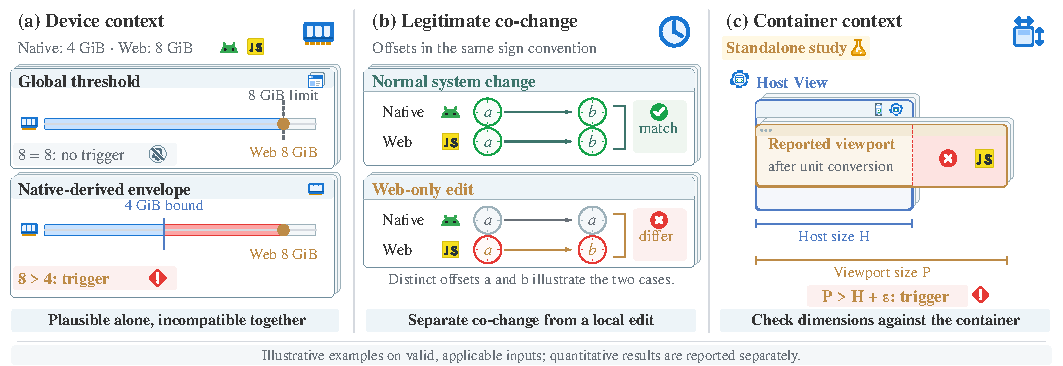
\includegraphics[width=\textwidth]{figures/HybridGuard_Fig3_mechanisms_v3.pdf}
  \caption{Illustrative mechanisms on applicable observations. (a) A Web report of 8 GiB stays within the fixed 8 GiB comparator but exceeds the envelope derived from Native memory of 4 GiB. (b) After offsets are converted to the same sign convention, a normal system change moves Native and Web together, whereas a Web-only edit creates a mismatch. (c) A converted viewport dimension P exceeding the Host bound plus tolerance triggers the standalone geometry check. These schematics add no measured records.}
  \label{fig:mechanisms}
  \Description{Three illustrative panels show a Native memory bound, legitimate timezone co-change versus a Web-only change, and a standalone Host geometry bound.}
\end{figure*}

